\section{Unsupervised Analysis}
\subsection{Principal Component Analysis}
The preprocessed data are then centered and scaled. Principal component analysis (PCA) is performed on the centered and scaled matrix of the \(165\) retained predictors, so that the decomposition is driven by the correlation structure rather than by the original measurement scales.

If \(\lambda_k\) denotes the \(k\)-th eigenvalue of the correlation matrix, the proportion of explained inertia associated with axis \(k\) is given by
\begin{equation}
\frac{\lambda_k}{\sum_{j=1}^{165}\lambda_j}.
\label{eq:pca_inertia_ratio}
\end{equation}

Numerically, the first two principal components explain \(29.79\%\) of the total inertia, the first four explain \(43.52\%\), the first ten explain \(59.01\%\), and the first \(34\) explain \(81.60\%\); these values are summarized in Appendix~\ref{app:skewness}, Subsection~\ref{subsec:pca_variable_space}, Table~\ref{tab:pca_subspace_summary}. Therefore, PCA reveals a nontrivial low-dimensional structure in the data. However, a substantial part of the total variability remains distributed across many directions, which limits the possibility of obtaining a clearly separated five-class visualization in only two dimensions. This limitation can also be observed by analyzing the quality of representation of the individuals. For an observation \(i\), the quality of representation on the first \(k\) principal axes is measured by the cumulative squared cosine:
\begin{equation}
\cos^2_i(1{:}k)=\sum_{s=1}^k \cos^2_i(s).
\label{eq:pca_cumulative_cos2}
\end{equation}

The mean value of this quantity is \(0.2888\) on the first two axes, \(0.4283\) on the first four axes, \(0.5900\) on the first ten axes, and \(0.8064\) on the first \(34\) axes; see again Table~\ref{tab:pca_subspace_summary}. Hence, the first principal plane captures less than one third of the total information for a typical observation, whereas a substantially better representation is obtained only when considering a higher-dimensional subspace. A similar limitation is observed in the variable space. The analysis of the cumulative squared cosines shows that only a limited subset of variables is well represented on the first principal plane; see Appendix~\ref{app:skewness}, Tables~\ref{tab:pca_best_plane12} and~\ref{tab:pca_representation_counts}. Although the representation improves when the first four principal axes are considered, a large part of the predictor set still requires a higher-dimensional subspace to be properly projected; see Tables~\ref{tab:pca_best_first4} and~\ref{tab:pca_representation_counts}. Consequently, the interpretation of the PCA should not rely exclusively on the first two-dimensional representation, but should also account for higher-dimensional principal subspaces.
In the first principal plane, the variables with the largest contributions include several descriptors from the spectrum envelope family; see Appendix~\ref{app:skewness}, Table~\ref{tab:pca_pc1_variables}. This suggests that the first principal axis represents a strong contrast mainly associated with these descriptors.

On the second principal axis, the most contributive variables are dominated by variability descriptors and by variables related to temporal features, such as threshold and zero-crossing descriptors; see Table~\ref{tab:pca_pc2_variables}. Therefore, the second axis of the principal plane can be interpreted as being more clearly associated with temporal crossing features and variability-related descriptors.

The relationships between the principal axes of the second plane and the variables of interest are weaker. Nevertheless, the third principal axis still shows an association with temporal crossing features and variability descriptors; see Table~\ref{tab:pca_pc3_variables}. In contrast, the fourth principal axis appears to represent an opposition between certain \texttt{ASE} variables and \texttt{SFM}/\texttt{SFMV} variables, that is, between part of the audio spectrum envelope information and part of the spectral flatness information; see Table~\ref{tab:pca_pc4_variables}.

The first two principal planes are displayed jointly in Fig.~\ref{fig:pca_principal_planes}. From these figures and from the results discussed above, it can be concluded that the first two principal planes are not sufficient to provide an adequate representation of either the individuals or the variables. Although the dataset exhibits a nontrivial underlying structure, this structure is not strongly concentrated in a very low-dimensional subspace. The first principal plane, shown in panel (a) of Fig.~\ref{fig:pca_principal_planes}, reveals a partial horizontal contrast. \textit{Pop} observations are more frequently located on the positive side of the first principal component, whereas \textit{Classical} observations tend to be more concentrated on the negative side. \textit{Rock} also tends to occupy the lower-right region of the plane. However, the point clouds remain broad and strongly overlapping, indicating that the first principal plane does not provide a sharp discrimination among the five musical genres. The second principal plane, shown in panel (b) of Fig.~\ref{fig:pca_principal_planes}, provides additional information, but it does not eliminate the overlap between genres. Overall, the PCA confirms that the dataset contains relevant multivariate structure. Nevertheless, this structure is not organized into five clearly separated linear groups, which limits the discriminative power of a purely two-dimensional PCA visualization.

\begin{figure}[!t]
\centering
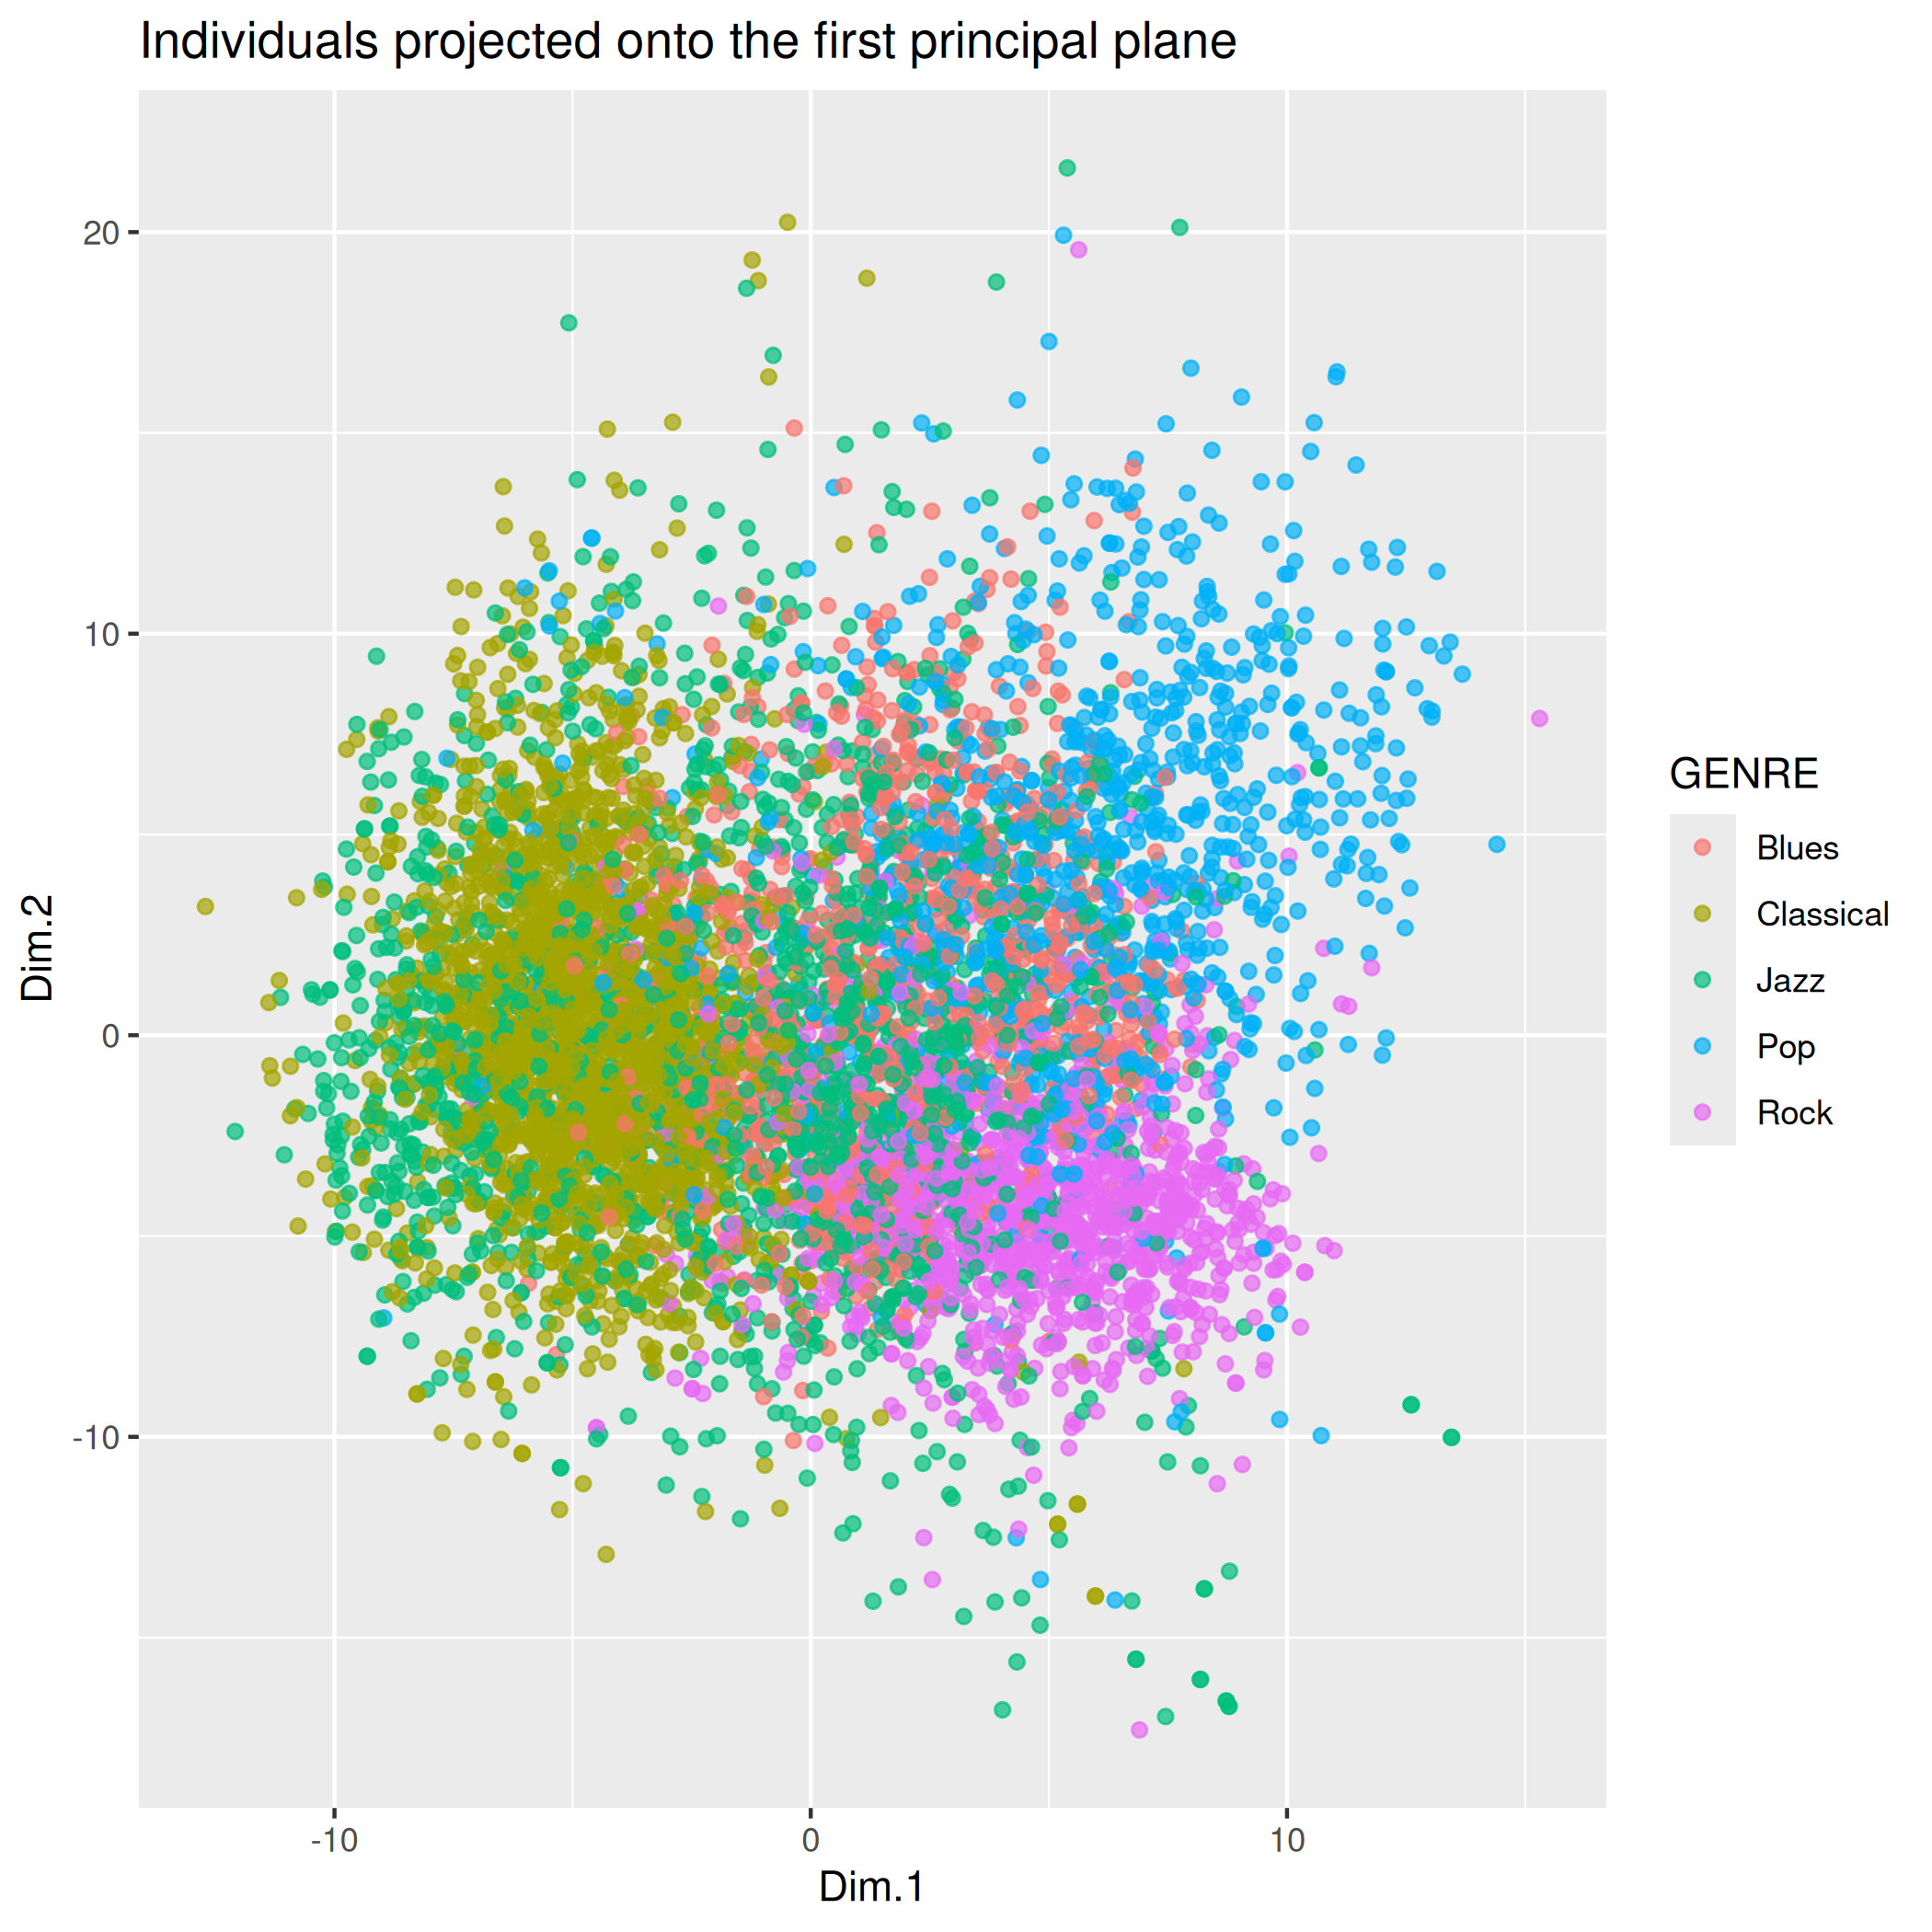
\includegraphics[width=\columnwidth]{../output/part1/pca_first_plane.png}

\vspace{2pt}
\footnotesize{(a) First principal plane \((\mathrm{PC1},\mathrm{PC2})\).}

\vspace{4pt}
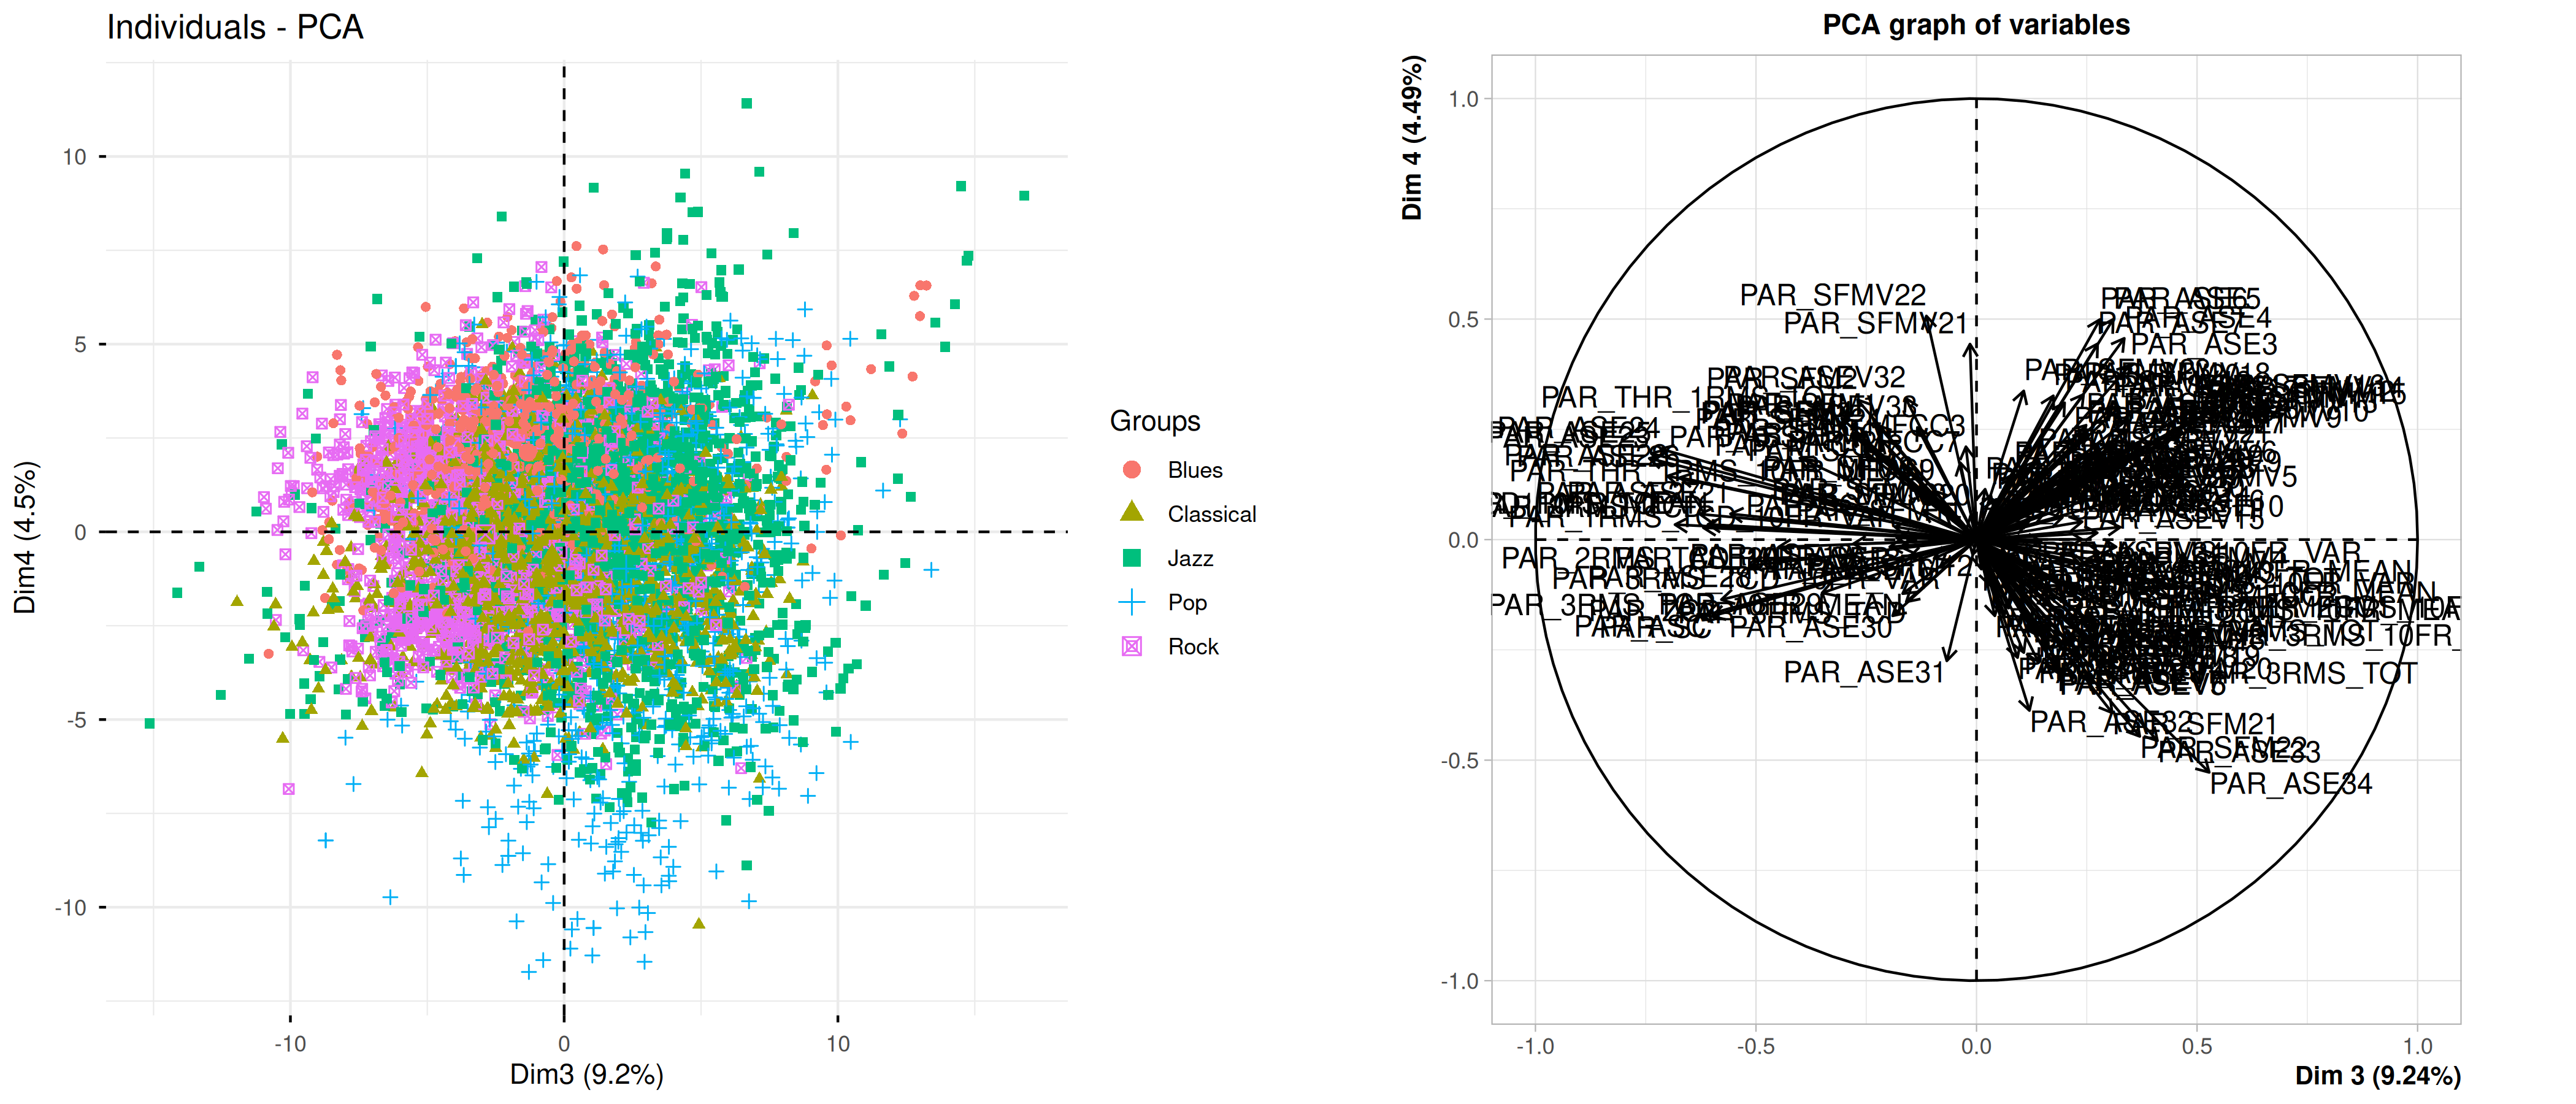
\includegraphics[width=\columnwidth]{../output/part1/pca_second_plane.png}

\vspace{2pt}
\footnotesize{(b) Second principal plane \((\mathrm{PC3},\mathrm{PC4})\).}

\caption{Composite representation of the two principal planes used in the unsupervised analysis.}
\label{fig:pca_principal_planes}
\end{figure}
